%% Exercice 2

%\ExoSpecs{\TTBF{CalculTVA.sh}}{\TTBF{\RenduDir/src/exo1/}}{750}{640}{\TTBF{write}}
\ExoSpecsCustom{\TTBF{queue\_linked\_list.c}}{\TTBF{\RenduDir/src/}}{750}{640}{Fonctions autorisées}{\TTBF{malloc(3)}, \TTBF{free(3)}, \TTBF{memcpy(3)}, \TTBF{printf(3)}}

\vspace*{0.7cm}

\noindent \ExoObjectif{Le but de l'exercice est d'implémenter une file en C à base de liste chaînée.}

\bigskip

\noindent Les fonctions demandées dans cet exercice devront se trouver dans une bibliothèque nommée \TTBF{libmyqueue}.
Après un appel à la commande \texttt{make} à la racine du projet, il faut que votre chaîne de compilation produise à la racine de votre projet une version statique de la bibliothèque (qui se nommera \TTBF{libmyqueue.a}) ainsi qu'une version dynamique de la bibliothèque (qui se nommera \TTBF{libmyqueue.so}).

\bigskip

\noindent Vous devez écrire plusieurs fonctions permettant de créer, utiliser, vider, et libérer une file.
Un fichier \TTBF{queue\_linked\_list.h} contenant toutes les fonctions exportables à implémenter vous est fourni en annexe.
Vous devez déclarer une structure \TTBF{queue\_ll} et l'ajouter dans \TTBF{queue\_linked\_list.h}.
N'oubliez pas de déclarer également une structure qui contiendra les éléments de la liste chaînée.
Pour les premières étapes, vous devrez implémenter une version simplifiée de la file qui ne prend en charge que des entiers positifs.

\bigskip

\noindent Conceptuellement, les fonctions manipulant des files de type \TTBF{queue\_ll*} devront pouvoir gérer ces 3 cas :

\bigskip

\begin{center}
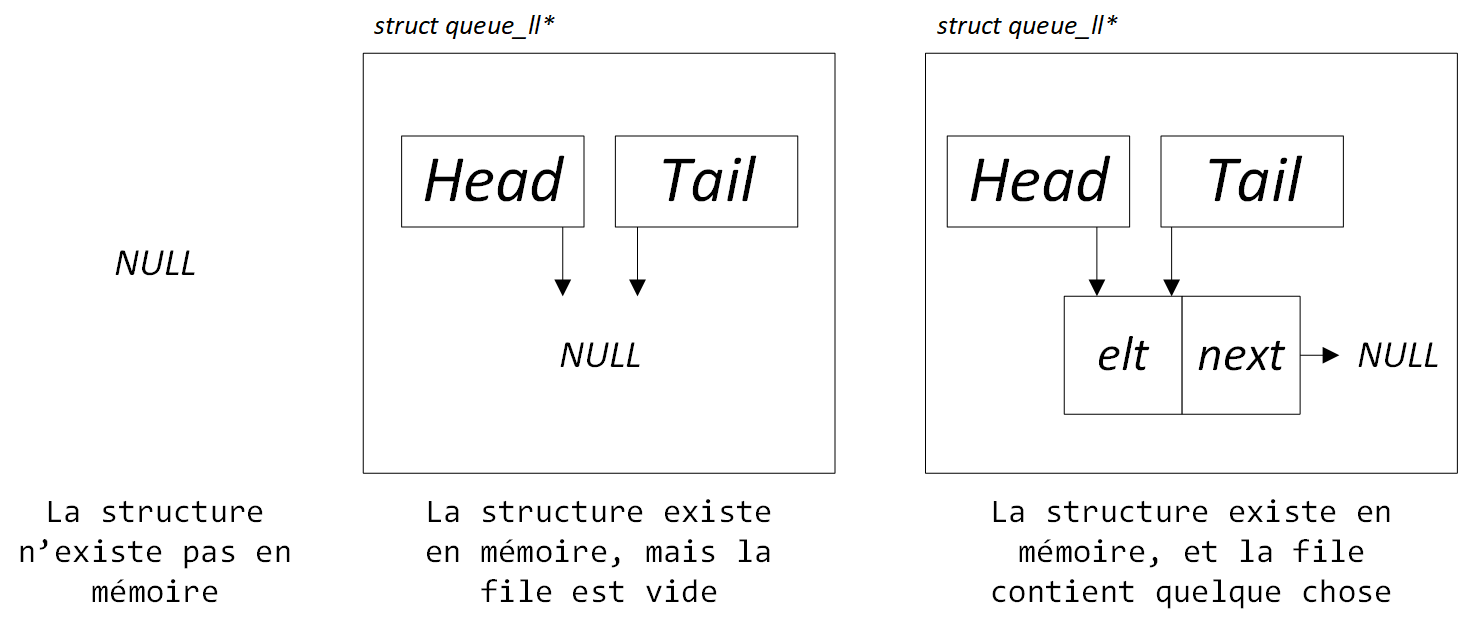
\includegraphics[scale=0.85]{Cours/Files_Implementation_LL.png}
\end{center}

%\bigskip
\newpage

%\noindent Vous devez implémenter les 11 fonctions suivantes :
%\begin{itemize}
%\item \TTBF{queue\_ll *queue\_ll\_create(void)}
%\item \TTBF{void queue\_ll\_delete(queue\_ll *queue)}
%\item \TTBF{int queue\_ll\_length(queue\_ll *queue)}
%\item \TTBF{int queue\_ll\_enqueue(int elt, queue\_ll *queue)}
%\item \TTBF{int queue\_ll\_dequeue(queue\_ll *queue)}
%\item \TTBF{int queue\_ll\_head(queue\_ll *queue)}
%\item \TTBF{int queue\_ll\_tail(queue\_ll *queue)}
%\item \TTBF{int queue\_ll\_clear(queue\_ll *queue)}
%\item \TTBF{int queue\_ll\_is\_empty(queue\_ll *queue)}
%\item \TTBF{int queue\_ll\_insert(int elt, int pos, queue\_ll *queue)}
%\item \TTBF{int queue\_ll\_replace(int elt, int pos, queue\_ll *queue)}
%\item \TTBF{int queue\_ll\_search(int elt, queue\_ll *queue)}
%\item \TTBF{queue\_ll *queue\_ll\_reverse(queue\_ll *queue)}
%\item \TTBF{void queue\_ll\_print(queue\_ll *queue)}
%\end{itemize}

\noindent Vous devez implémenter les fonctions suivantes :

\bigskip

\lstset{language=C}
\begin{lstlisting}[frame=single,title={Liste des fonctions pour une file avec liste chaînée}]
queue_ll *queue_ll_create(void);
void queue_ll_delete(queue_ll *queue);

int queue_ll_length(queue_ll *queue);

int queue_ll_enqueue(int elt, queue_ll *queue);
int queue_ll_dequeue(queue_ll *queue);
int queue_ll_head(queue_ll *queue);
int queue_ll_tail(queue_ll *queue);

int queue_ll_clear(queue_ll *queue);
int queue_ll_is_empty(queue_ll *queue);

int queue_ll_insert(int elt, int pos, queue_ll *queue);
int queue_ll_replace(int elt, int pos, queue_ll *queue);

int queue_ll_search(int elt, queue_ll *queue);
queue_ll *queue_ll_reverse(queue_ll *queue);
void queue_ll_print(queue_ll *queue);
\end{lstlisting}


\subsubsection*{\TTBF{queue\_ll *queue\_ll\_create(void)}}

\noindent Cette fonction crée une file vide.
En cas d'erreur (pas assez de mémoire), elle renvoie un pointeur \TTBF{NULL}.


\subsubsection*{\TTBF{void queue\_ll\_delete(queue\_ll *queue)}}

\noindent Cette fonction vide une file de l'ensemble de ses éléments, et détruit la structure restante.
Si le paramètre donné est \TTBF{NULL}, la fonction ne fait rien.


\subsubsection*{\TTBF{int queue\_ll\_length(queue\_ll *queue)}}

\noindent Cette fonction renvoie la longueur de la file (c'est-à-dire le nombre d'éléments actuellement dans la file).
Si le paramètre donné est \TTBF{NULL}, la fonction renvoie $ -1 $.


\subsubsection*{\TTBF{int queue\_ll\_enqueue(int elt, queue\_ll *queue)}}

\noindent Cette fonction enfile un élément dans une file, c'est-à-dire qu'elle ajoute un élément en queue.
En cas de succès, la fonction renvoie $ 0 $.
Si la file donnée en paramètre est \TTBF{NULL}, la fonction renvoie $ -1 $.
Si le nombre donné en paramètre est inférieur à $ 0 $, la fonction renvoie $ -4 $.
S'il y a un problème de mémoire, la fonction renvoie $ -3 $.


\subsubsection*{\TTBF{int queue\_ll\_dequeue(queue\_ll *queue)}}

\noindent Cette fonction défile un élément d'une file, c'est-à-dire qu'elle supprime l'élément en tête.
En cas de succès, la fonction renvoie $ 0 $.
Si la file donnée en paramètre est \TTBF{NULL}, la fonction renvoie $ -1 $.
Si la file donnée en paramètre est vide, la fonction renvoie $ -2 $.


\subsubsection*{\TTBF{int queue\_ll\_head(queue\_ll *queue)}}

\noindent Cette fonction renvoie l'élément en tête de file.
Si la file donnée en paramètre est \TTBF{NULL}, la fonction renvoie $ -1 $.
Si la file donnée en paramètre est vide, la fonction renvoie $ -2 $.


\subsubsection*{\TTBF{int queue\_ll\_tail(queue\_ll *queue)}}

\noindent Cette fonction renvoie l'élément en queue de file.
Si la file donnée en paramètre est \TTBF{NULL}, la fonction renvoie $ -1 $.
Si la file donnée en paramètre est vide, la fonction renvoie $ -2 $.


\subsubsection*{\TTBF{int queue\_ll\_clear(queue\_ll *queue)}}

\noindent Cette fonction vide une file de l'ensemble de ses éléments, sans détruire la structure de la file.
La fonction renvoie le nombre d'éléments supprimés de la mémoire.
Si le paramètre donné est \TTBF{NULL}, la fonction renvoie $ -1 $.
Si la file donnée en paramètre est vide, la fonction renvoie $ 0 $.


\subsubsection*{\TTBF{int queue\_ll\_is\_empty(queue\_ll *queue)}}

\noindent Cette fonction teste si une file est vide ou non.
Si la file est vide, la fonction renvoie $ 1 $.
Si la file n'est pas vide, la fonction renvoie $ 0 $.
Si la file donnée en paramètre est \TTBF{NULL}, la fonction renvoie $ -1 $.


\subsubsection*{\TTBF{int queue\_ll\_insert(int elt, int pos, queue\_ll *queue)}}

\noindent Cette fonction ajoute un élément dans la file à l'emplacement \textit{pos}.
La première position est celle où l'élément le plus ancien a été placé (c'est-à-dire la tête de la file), cette position sera numérotée $ 0 $.
L'ancien élément qui était présent à cette position est décalé d'un cran en arrière (vers la queue).
Si le nombre donné en paramètre est inférieur à $ 0 $, la fonction renvoie $ -4 $.
Si l'emplacement n'existe pas et est positif, on ajoute l'élément en queue.
Si l'emplacement n'existe pas et est négatif, on ajoute l'élément en tête.
En cas de succès, la fonction renvoie $ 0 $.
Si la file donnée en paramètre est \TTBF{NULL}, la fonction renvoie $ -1 $.
%Si la file donnée en paramètre est vide, la fonction renvoie $ -2 $.
S'il y a un problème de mémoire, la fonction renvoie $ -3 $.


\subsubsection*{\TTBF{int queue\_ll\_replace(int elt, int pos, queue\_ll *queue)}}

\noindent Cette fonction remplace un élément dans la file à l'emplacement \textit{pos}, et renvoie l'élément qui était présent à cet endroit.
La première position est celle où l'élément le plus ancien a été placé (c'est-à-dire la tête de la file), cette position sera numérotée $ 0 $.
Si le nombre donné en paramètre est inférieur à $ 0 $, la fonction renvoie $ -4 $.
Si l'emplacement n'existe pas et est positif, on remplace l'élément en queue.
Si l'emplacement n'existe pas et est négatif, on remplace l'élément en tête.
%En cas de succès, la fonction renvoie $ 0 $.
Si la file donnée en paramètre est \TTBF{NULL}, la fonction renvoie $ -1 $.
Si la file donnée en paramètre est vide, la fonction renvoie $ -2 $.


\subsubsection*{\TTBF{int queue\_ll\_search(int elt, queue\_ll *queue)}}

\noindent Cette fonction recherche un élément dans la file et renvoie sa position dans la liste chaînée.
La première position est celle où l'élément le plus ancien a été placé (c'est-à-dire la tête de la file), cette position sera numérotée $ 0 $.
Si l'élément n'est pas trouvé, la fonction renvoie $ -4 $.
Si la file donnée en paramètre est \TTBF{NULL}, la fonction renvoie $ -1 $.


\subsubsection*{\TTBF{queue\_ll *queue\_ll\_reverse(queue\_ll *queue)}}

\noindent Cette fonction inverse la position de tous les éléments de la file.
Le premier élément devient le dernier, l'avant dernier devient le deuxième, etc.
En cas de succès, la fonction renvoie le pointeur vers l'éventuelle nouvelle adresse en mémoire de la structure de la file inversée.
En cas de problème mémoire, on renvoie \TTBF{NULL}, et l'ancienne file doit rester à son ancienne adresse mémoire sans subir la moindre modification.
Si la file donnée en paramètre est \TTBF{NULL}, la fonction renvoie \TTBF{NULL}.


\subsubsection*{\TTBF{void queue\_ll\_print(queue\_ll *queue)}}

\noindent Cette fonction affiche le contenu de la file.
Le format d'affichage attendu implique d'afficher un seul élément par ligne, suivi d'un retour à la ligne.
L'élément en tête de file sera affiché en premier.
Si la file donnée en paramètre est vide, seul un retour à la ligne est affiché.
Si la file donnée en paramètre est \TTBF{NULL}, rien n'est affiché.

\bigskip

\lstset{language=sh}
\begin{lstlisting}[frame=single,title={Exemple d'affichage du cas normal : file contenant 42, 5, 13}]
$ ./my_queue_linked_list
42
5
13

$
\end{lstlisting}

\bigskip

\lstset{language=sh}
\begin{lstlisting}[frame=single,title={Exemple d'affichage d'une file vide}]
$ ./my_queue_linked_list

$
\end{lstlisting}

\bigskip

\lstset{language=sh}
\begin{lstlisting}[frame=single,title={Exemple d'affichage d'un pointeur NULL}]
$ ./my_queue_linked_list
$
\end{lstlisting}